%%%%%%%%%%%%%%%%%%%%%%%%%%%%%%%%%%%%%%%%%
% Beamer Presentation
% LaTeX Template
% Version 1.0 (10/11/12)
%
% This template has been downloaded from:
% http://www.LaTeXTemplates.com
%
% License:
% CC BY-NC-SA 3.0 (http://creativecommons.org/licenses/by-nc-sa/3.0/)
%
%%%%%%%%%%%%%%%%%%%%%%%%%%%%%%%%%%%%%%%%%

%----------------------------------------------------------------------------------------
%	PACKAGES AND THEMES
%----------------------------------------------------------------------------------------

\documentclass{beamer}

\mode<presentation> {

% The Beamer class comes with a number of default slide themes
% which change the colors and layouts of slides. Below this is a list
% of all the themes, uncomment each in turn to see what they look like.

%\usetheme{default}
%\usetheme{AnnArbor}
%\usetheme{Antibes}
%\usetheme{Bergen}
%\usetheme{Berkeley}
%\usetheme{Berlin}
%\usetheme{Boadilla}
%\usetheme{CambridgeUS}
%\usetheme{Copenhagen}
%\usetheme{Darmstadt}
%\usetheme{Dresden}
%\usetheme{Frankfurt}
%\usetheme{Goettingen}
%\usetheme{Hannover}
%\usetheme{Ilmenau}
%\usetheme{JuanLesPins}
%\usetheme{Luebeck}
\usetheme{Madrid}
%\usetheme{Malmoe}
%\usetheme{Marburg}
%\usetheme{Montpellier}
%\usetheme{PaloAlto}
%\usetheme{Pittsburgh}
%\usetheme{Rochester}
%\usetheme{Singapore}
%\usetheme{Szeged}
%\usetheme{Warsaw}

% As well as themes, the Beamer class has a number of color themes
% for any slide theme. Uncomment each of these in turn to see how it
% changes the colors of your current slide theme.

%\usecolortheme{albatross}
%\usecolortheme{beaver}
%\usecolortheme{beetle}
%\usecolortheme{crane}
%\usecolortheme{dolphin}
%\usecolortheme{dove}
%\usecolortheme{fly}
%\usecolortheme{lily}
%\usecolortheme{orchid}
%\usecolortheme{rose}
%\usecolortheme{seagull}
%\usecolortheme{seahorse}
%\usecolortheme{whale}
%\usecolortheme{wolverine}

%\setbeamertemplate{footline} % To remove the footer line in all slides uncomment this line
%\setbeamertemplate{footline}[page number] % To replace the footer line in all slides with a simple slide count uncomment this line

%\setbeamertemplate{navigation symbols}{} % To remove the navigation symbols from the bottom of all slides uncomment this line
}

\usepackage{graphicx} % Allows including images
\usepackage[absolute, overlay]{textpos}
\usepackage{booktabs} % Allows the use of \toprule, \midrule and \bottomrule in tables
\usepackage{tikz}
\usetikzlibrary{positioning,calc,backgrounds,shapes}

\usepackage[labelformat=empty]{caption}
\captionsetup{compatibility=false}

\tikzset{My Arrow Style/.style={single arrow, fill=red!30, anchor=base, align=center,text width=4cm}}
\newcommand{\arrowthis}[2][]{\tikz[baseline] \node [My Arrow Style,#1] {#2};}


\tikzset{My Speech Style/.style={ellipse callout, fill=red!50, anchor=base, align=center,text width=2.8cm}}
\newcommand{\speechthis}[2][]{
    \tikz[baseline]{\node[My Speech Style, #1]{#2};}
}%

\newcommand{\source}[1]{\begin{textblock*}{4cm}(8.7cm,8.2cm)
        \begin{beamercolorbox}[ht=0.5cm,right]{framesource}
        \usebeamerfont{framesource}\usebeamercolor[fg]{framesource} Source: {#1}
        \end{beamercolorbox}
    \end{textblock*}
}
%----------------------------------------------------------------------------------------
%	TITLE PAGE
%----------------------------------------------------------------------------------------

\title[Universitatea din Bucure\c{s}ti]{Aplica\c{t}ii ale Schemelor de Partajare a Secretelor}

% The short title appears at the bottom of every slide, the full title is only on the title page
%An Immediate Multi-Party Generalization of ID-NIKE from Constrained PRF
\author[Drago\c{s} Alin Rotaru]{Drago\c{s} Alin Rotaru} % Your name
\institute[UniBuc] % Your institution as it will appear on the bottom of every slide, may be shorthand to save space
{
Universitatea din Bucure\c{s}ti\\ % Your institution for the title page
% \medskip
% \textit{ruxandra.olimid@fmi.unibuc.ro, r.dragos0@gmail.com} % Your email address
}
\date{9 februarie, 2015} % Date, can be changed to a custom date

\begin{document}

\begin{frame}
\titlepage % Print the title page as the first slide
\end{frame}


%----------------------------------------------------------------------------------------
%	PRESENTATION SLIDES
%----------------------------------------------------------------------------------------

%------------------------------------------------
\section{Overview} % Sections can be created in order to organize your presentation into discrete blocks, all sections and subsections are automatically printed in the table of contents as an overview of the talk
%------------------------------------------------

\subsection{Motiva\c{t}ie}
\begin{frame}
    \frametitle{Motiva\c{t}ie: scheme de partajare} % Table of contents slide, comment this block out to remove it
    \only<1-2>{
        \begin{textblock*}{4cm}(3cm, 3cm)
        \begin{figure}
            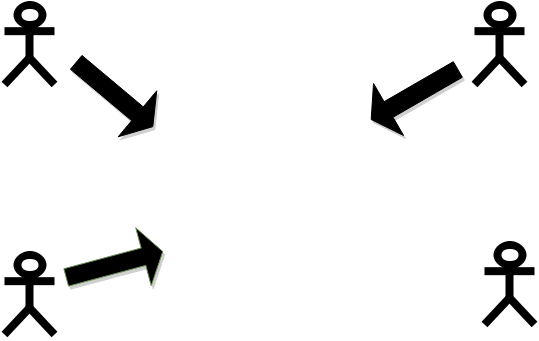
\includegraphics[width=7cm,height=7cm,keepaspectratio]{img/motivation/key1.png}
        \end{figure}
        \end{textblock*}
    }
    \only<2> {
        \begin{textblock*}{4cm}(4.5cm, 4cm)
        \begin{figure}
            
\includegraphics[width=2cm,height=2cm,keepaspectratio]{img/motivation/Lock.png}
        \end{figure}
        \end{textblock*}
    }
    \only<3-> {
        \begin{textblock*}{4cm}(3cm, 3cm)
        \begin{figure}
            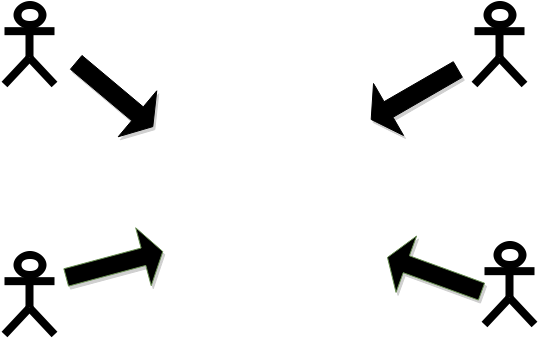
\includegraphics[width=7cm,height=7cm,keepaspectratio]{img/motivation/all_in.png}
        \end{figure}
        \end{textblock*}

        \begin{textblock*}{4cm}(4.5cm, 4cm)
        \begin{figure}
            
\includegraphics[width=2cm,height=2cm,keepaspectratio]{img/motivation/key-128.png}
        \end{figure}
        \end{textblock*}
    }
\end{frame}

\begin{frame}
    \frametitle{Motiva\c{t}ie: sisteme de stocare} 
    \only<1-2> {

        \begin{textblock*}{2cm}(1cm, 4.7cm)
        \begin{figure}
            
\includegraphics[width=2cm,height=2cm,keepaspectratio]{img/motivation/boy-128.png}
        \end{figure}
        \end{textblock*}
    }
    \only<2-2> {

        \begin{textblock*}{4cm}(4cm, 2cm)
        \begin{figure}
            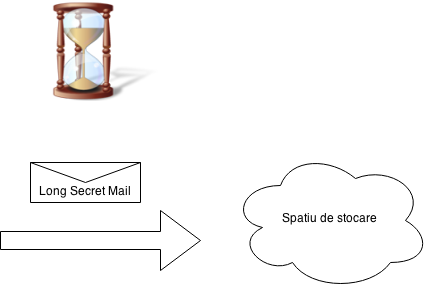
\includegraphics[width=7cm,height=7cm,keepaspectratio]{img/motivation/storage-system.png}
        \end{figure}
        \end{textblock*}
    }
    \only<3-> {

        \begin{textblock*}{2cm}(1cm, 4.7cm)
        \begin{figure}
            
\includegraphics[width=2cm,height=2cm,keepaspectratio]{img/motivation/old-128.png}
        \end{figure}
        \end{textblock*}
    }
    \only<3-> {

        \begin{textblock*}{4cm}(4cm, 2cm)
        \begin{figure}
            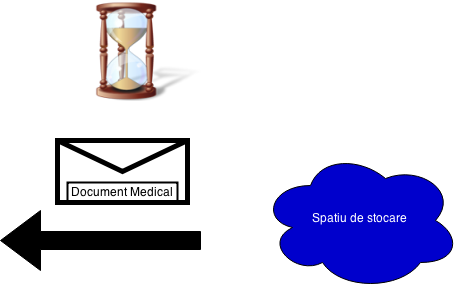
\includegraphics[width=7cm,height=7cm,keepaspectratio]{img/motivation/after_system.png}
        \end{figure}
        \end{textblock*}
    }
\end{frame}

%------------------------------------------------
\section{Scheme de partajare}

\begin{frame}
    \frametitle{Schema Shamir - intui\c{t}ie}
    \begin{itemize}
        \item $k$ puncte distincte \^{i}n plan definesc o curb\u{a} polinomial\u{a} unic\u{a} av\^{a}nd acelasi grad
        \pause
        \item Mai pu\c{t}in de $k$ puncte nu pot reconstitui polinomul original
    \end{itemize}
    \pause
    \only<3-> {
        \begin{textblock*}{4cm}(5cm, 5cm)
        \begin{figure}
            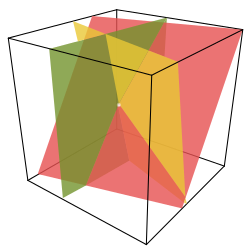
\includegraphics[width=3.5cm,height=3.5cm,keepaspectratio]{img/shamir/shamir.png}
       \end{figure}
        \end{textblock*}
     }
\end{frame}

\begin{frame}
    \frametitle{Schema Shamir}
    \begin{itemize}
        \item Secret $\mathcal{S}$
        \pause
        \item Schema $(k,n)$ majoritar\u{a}
        \pause
        \item Oricare $k$ participan\c{t}i din cei $n$ pot reconstitui $\mathcal{S}$
        \pause
        \item Mai pu\c{t}in de $k$ participan\c{t}i nu ob\c{t}in nici o informa\c{t}ie despre $\mathcal{S}$
        \pause
        \item Se alege un polinom $f$ de grad $k$ av\^{a}nd coeficien\c{t}i aleatori, termenul liber fiind $\mathcal{S}$
        \pause
        \item Participantul $P_i$ primeste $f(i)$, $i = \{1, 2, ...n\}$
        \pause
        \item Dupa reconstituire secretul $\mathcal{S}$ se afla \^{i}n $f(0)$.
    \end{itemize}
\end{frame}

\begin{frame}
    \frametitle{Schema Shamir}
    \only<1> {
        \begin{exampleblock}{Example}
           Se consider\u{a} 8 participan\c{t}i, unde oricare $3$ pot reconstitui secretul $\mathcal{S}$. Fie polinomul $f(x) = 20x ^ 3 + 14x ^ 2 + 31x + S$
        \end{exampleblock}
    }
    \only<2> {
     \begin{textblock*}{4cm}(3.5cm, 2cm)
        \begin{figure}
            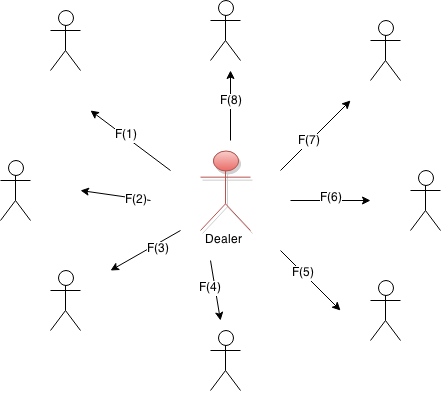
\includegraphics[width=6cm,height=6cm,keepaspectratio]{img/shamir/example.png}
       \end{figure}
        \end{textblock*}
 
    }
\end{frame}

\begin{frame}
    \frametitle{Schema unanim\u{a} XOR}
    \begin{itemize}
        \item Schema majoritar\u{a} $(n,n)$.
        \pause
        \item $n-1$ participan\c{t}i primesc numere aleatoare: $s_1, s_2, \dots s_{n-1}$.
        \pause
        \item Cel de-al $n$-lea participant prime\c{s}te $S \oplus s_1 \oplus s_2 \oplus \dots \oplus s_{n-1}$.
    \end{itemize}
\end{frame}

\begin{frame}
    \frametitle{Schema Ito, Saito \c{s}i Nishizeki}

    \only<1-> {
    \begin{itemize}
        \item Schema Shamir e insuficient\u{a} pentru a realiza partajarea lui $\mathcal{S}$ unui grup particular de participan\c{t}i.
    \end{itemize}
    }
    \only<2-> {
        \begin{textblock*}{4cm}(3.5cm, 5cm)
            \begin{figure}
                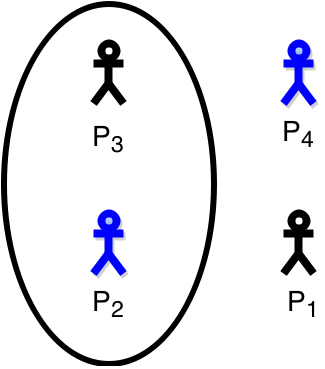
\includegraphics[width=3.5cm,height=3.5cm,keepaspectratio]{img/shamir/Ito.png}
           \end{figure}
        \end{textblock*}
    }
\end{frame}

%------------------------------------------------
\section{Sisteme de stocare}

\begin{frame}
    \frametitle{Asigurarea disponibilt\u{a}\c{t}ii cu ajutorul sistemelor RAID} 
\end{frame}
\end{document}
